\section{帧差分}

\subsection{帧间差分法简介}


当视频中存在移动物体的时候,相邻帧(或相邻三帧)之间在灰度上会有差别,求取两帧图像灰度差的绝对值,当绝对值超过一定阈值时,即可判断为运动目标,从而实现运动目标的检测功能



\subsection{双帧差分法}

记录视频序列中的第$n$帧和第$n-1$帧的图像为$I_n$和$I_{n-1}$

两帧对应像素点的灰度值记为$I_n(i,j)$和$I_{n-1}(i,j)$,将两帧图像对应像素点的灰度值进行相减,并取其绝对值,得到差分图像$D_n$

\begin{equation}
    D_n (i, j) = \left\lvert I_n (i, j) - I_{n - 1} (i, j) \right\rvert
\end{equation}

设定阈值$T$,逐个对像素点进行二值化处理,得到二值化图像$M_n'$。其中,灰度值为$255$的点即为前景(运动目标)点,灰度值为$0$的点即为背景点;最终可得到含有完整运动目标的图像$M_n$。

\begin{figure}
    \centering
    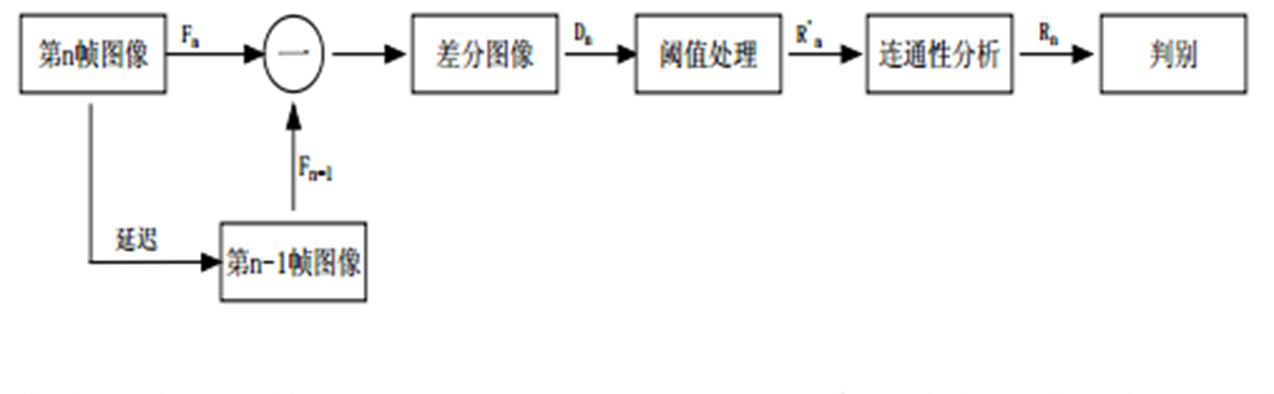
\includegraphics[width=0.618\textwidth]{images/fd_double.png}
    \caption{双帧差分示意图}
\end{figure}



\subsection{三帧差分法}

三帧差分法与双帧差分法类似,取相邻三帧按照下式计算,多进行一次``与''操作

\begin{equation}
    D_n (i, j) = \left\lvert I_{n - 1} (i, j) - I_n (i, j) \right\rvert \times \left\lvert I_n(i, j) - I_{n + 1} (i, j) \right\rvert
\end{equation}
\begin{figure}
    \centering
    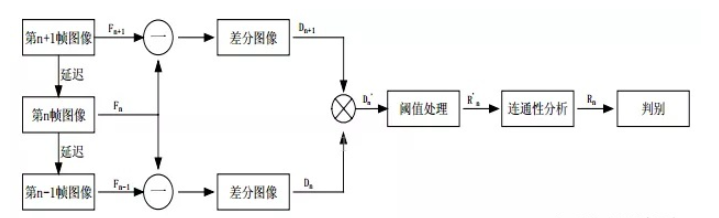
\includegraphics[width=0.618\textwidth]{images/fd_triple.png}
    \caption{三帧差分示意图}
\end{figure}



\subsection{OpenCV中实现帧差分法}

\begin{enumerate}
    \item 使用read函数得到当前帧的内容,absdiff函数可得到两帧绝对值的差,将所得图像阈值化,可得到目标图像。
    \item 使用findContours函数得到目标图像中物体轮廓,框选出运动物体。
\end{enumerate}

\begin{figure}
    \centering
    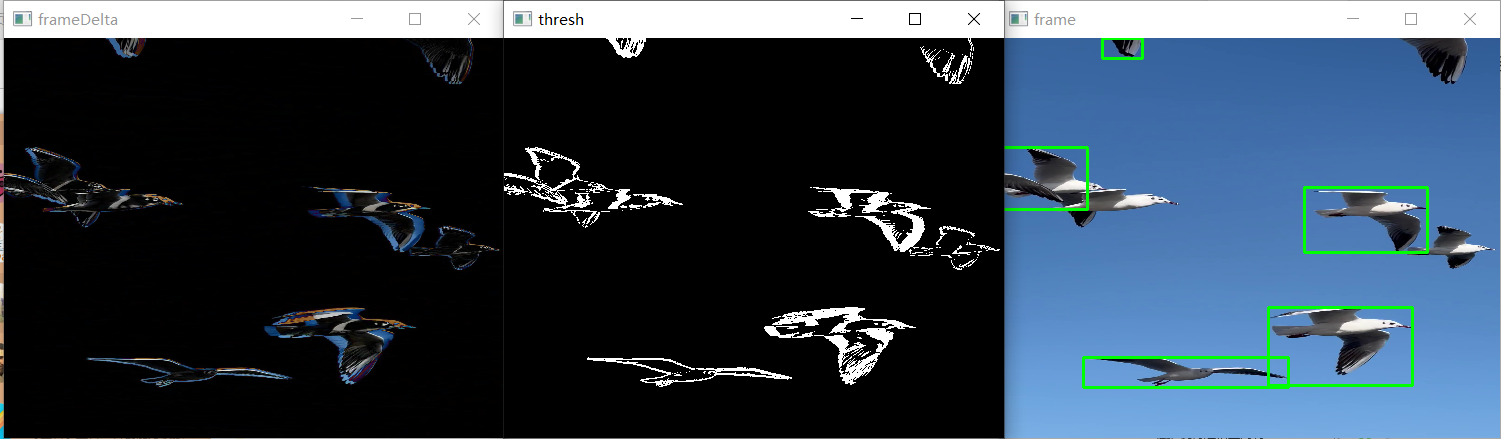
\includegraphics[width=0.618\textwidth]{images/frame_diff_bird.png}
    \caption{帧差分方法检测动态鸟的位置}
\end{figure}
